% This is the template for submission of abstracts to NetSci 2027 in DRESDEN, GERMANY.
% It is modified from NetSci2026.
% The editor of the booklet reserves the right to modify your submission.

% To process this file run LaTeX2e

% ******** DO NOT EDIT ****************
\documentclass[10pt]{article}
% \usepackage{mathptmx}
\usepackage[letterpaper,margin=20mm]{geometry}
\usepackage{graphicx}
\usepackage{lmodern}
\renewcommand{\familydefault}{\sfdefault}
\pagestyle{empty}
\setlength{\parskip}{0.25\baselineskip}
\renewcommand{\title}[1]{{\noindent\large\bfseries#1\medskip\\}}
\renewcommand{\author}[2]{{\noindent #1 \medskip\\ \noindent \small #2 \medskip\\}}
% *************************************

\newcommand{\ts}{\textsuperscript}

\begin{document}

% ********** USER DEFINED *************

\title{Scarce attention and the collapse of joint activity on social networks}
\author{
Alexei Vazquez\textsuperscript{1}
}
{
1. Nodes \& Links Ltd, Salisbury House, Station Road, Cambridge, CB1 2LA, UK\\
alexei@nodeslinks.com
}

Many of the things we do cannot be done alone. A meeting, a phone call or a
shared meal happens only if somebody else chooses it at the same moment. We must
decide how much priority to give it without knowing whether the other person
will turn up. Queueing models of human activity, which explain the bursty
timing of letters and emails [1,2], treat that priority as fixed. We let people
choose it [3]. Each person discounts the value of the joint activity by the risk
of being stood up, a risk learned from experience; being stood up costs time
that could have gone elsewhere.

This single change splits the behaviour into two phases. In one, partners keep
meeting. In the other, each has given up on the other, and since nobody offers,
nobody finds out that the other would have accepted. The switch between them is
abrupt and hard to undo: a pair that has stopped interacting does not restart on
its own, and recovery requires one side to keep trying, unanswered, for
roughly as long as the other takes to forget. The bursty activity patterns that
motivated the queueing models appear only close to this switch.

On a social network the scarce resource is attention. Somebody with many
contacts can give each of them only a small share of it, so beyond a critical
number of contacts no relationship can be sustained, however valuable. Ties
therefore fail first around the best-connected people, and the collapse spreads
through the network like a targeted attack on its hubs [4] --- except that no
attacker is needed, which makes networks with highly connected individuals
especially fragile. Simulations show that how many contacts a person has decides
which ties fail, while the local structure of the network decides how the
failures are arranged (Fig.~1): a network grown by introductions to friends of
friends breaks into isolated clusters, while the same network with its links
reshuffled loses as many ties but stays in one piece. For activities that need a
whole group to be present the limit tightens quickly with group size, giving a
largest group that can keep meeting. The theory thus derives, rather than
assumes, two facts observed in mobile-phone records: people keep only a limited
number of ties active [5], and ties decay when their usual rhythm is
interrupted [6].

\textbf{Acknowledgements.} All code is available at
github.com/av2atgh/interagents. The calculations were assisted by Claude
Opus~5, an AI assistant developed by Anthropic. Nodes \& Links Ltd provided
support in the form of salary for Alexei Vazquez but did not have any additional
role in the conceptualization of the study, the analysis, the decision to
publish or the preparation of the abstract.

\begin{figure}[!hb]
\begin{minipage}[t]{0.40\textwidth}
\vspace{0pt}
\small\raggedright\setlength{\parskip}{2pt}
\newcommand{\bibi}[1]{\par\noindent\hangindent=1.4em\hangafter=1 [#1]~}
\bibi{1}A.-L. Barab\'asi, Nature \textbf{435}, 207 (2005).
\bibi{2}J. G. Oliveira and A. Vazquez, Physica A \textbf{388}, 187 (2009).
\bibi{3}A. Vazquez, Phys.\ Rev.\ E \textbf{114}, 044322 (2026).
\bibi{4}R. Cohen, K. Erez, D. ben-Avraham and S. Havlin, Phys.\ Rev.\ Lett.\ \textbf{86}, 3682 (2001).
\bibi{5}G. Miritello, R. Lara, M. Cebri\'an and E. Moro, Sci.\ Rep.\ \textbf{3}, 1950 (2013).
\bibi{6}H. Navarro, G. Miritello, A. Canales and E. Moro, EPJ Data Sci.\ \textbf{6}, 31 (2017).

\medskip
\setlength{\parskip}{0pt}
\caption{\textbf{Local structure decides how joint activity collapses.}
Fraction of people in the largest cluster still linked by active ties, as the
cost of being stood up grows. A network grown by triadic closure (red)
fragments first; the same network with its links reshuffled (blue) keeps the
same fraction of active ties but stays connected longer, as does a
preferential-attachment network (green). 600 people, 4 contacts on average,
24 simulations per point.}
\end{minipage}\hfill
\begin{minipage}[t]{0.57\textwidth}
\vspace{0pt}
\centering
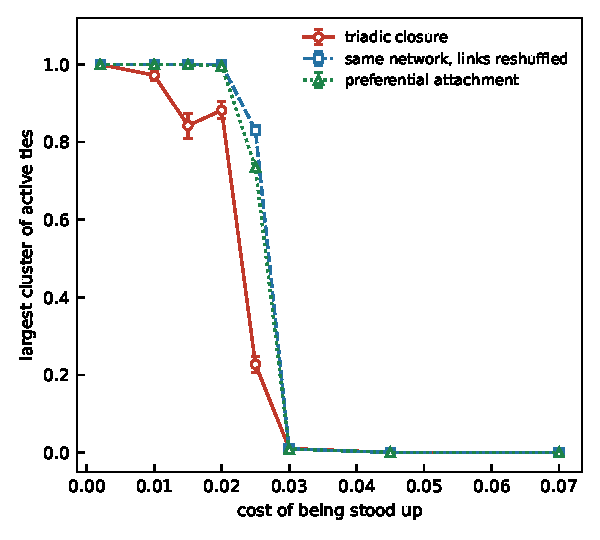
\includegraphics[width=\linewidth]{fig_netsci.pdf}
\end{minipage}
\end{figure}

% *************************************
\end{document}
